
% Conquest of Tlalocan chapter ----------------------------------------
\chapter*{Conquest of Tlalocan}
\addcontentsline{toc}{chapter}{Conquest of Tlalocan}

\begin{flushright}
\parbox{0.8\textwidth}{
\emph{The human mind is inspired enough when it comes to inventing
horrors; it is when it tries to invent a Heaven that it shows itself
cloddish. \\
\hspace*{\fill}{\textperiodcentered \textperiodcentered \textperiodcentered \hspace*{0.2em} Evelyn Waugh} } }
\end{flushright}

\noindent
Conquest of Tlalocan is chess variant which is played on 24 x 24 board,
with bright cyan and red fields and light green and dark red pieces.
Star colors are bright red and bright blue. In algebraic notation, columns
are enumerated from 'a' to 'x', and rows are enumerated from '1' to '24'.
A new piece is introduced, Shaman.

\textbf{\huge{TODO :: Star colors !!!}} % TODO :: FIX ME !!!

\clearpage % ..........................................................

\section*{Shaman}
\addcontentsline{toc}{section}{Shaman}

\noindent
\begin{wrapfigure}{l}{0.4\textwidth}
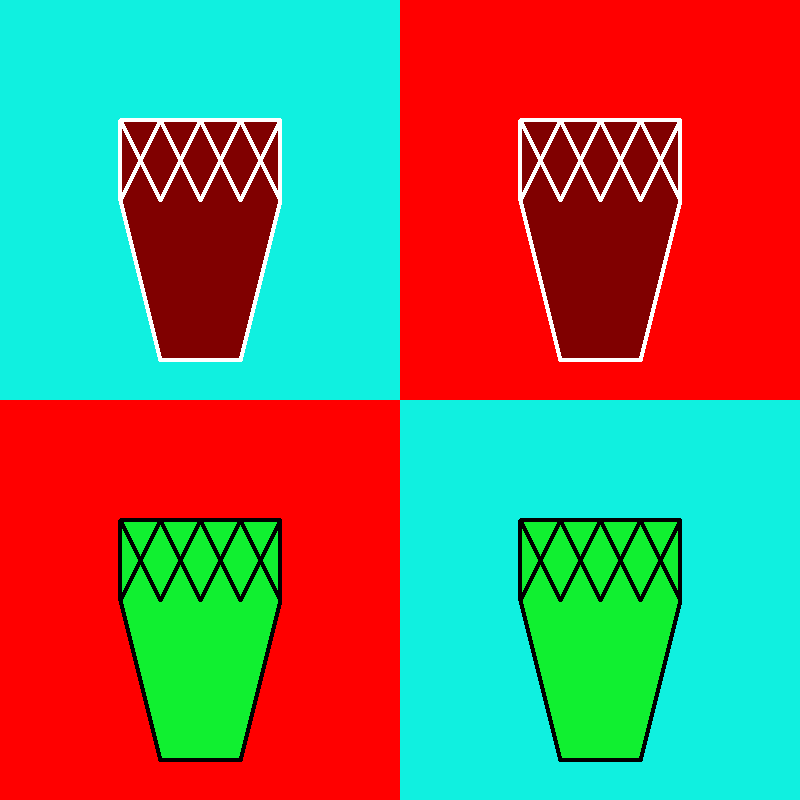
\includegraphics[width=0.4\textwidth, keepaspectratio=true]{pieces/14_shaman.png}
\caption{Shaman}
\label{fig:14_shaman}
% % \centering
\end{wrapfigure}


*** separate step-fields and capture-fields ***

Moves similar to Unicorn. For light Shaman, step-fields are as
Knight, capture-field are as long-range Unicorn. For dark one,
it's the opposite.

Trance-journey ...


\clearpage % ..........................................................

\section*{Initial setup}
\addcontentsline{toc}{section}{Initial setup}

Initial setup can be seen in image below:

\noindent
% \begin{figure}[t]
\begin{figure}[h]
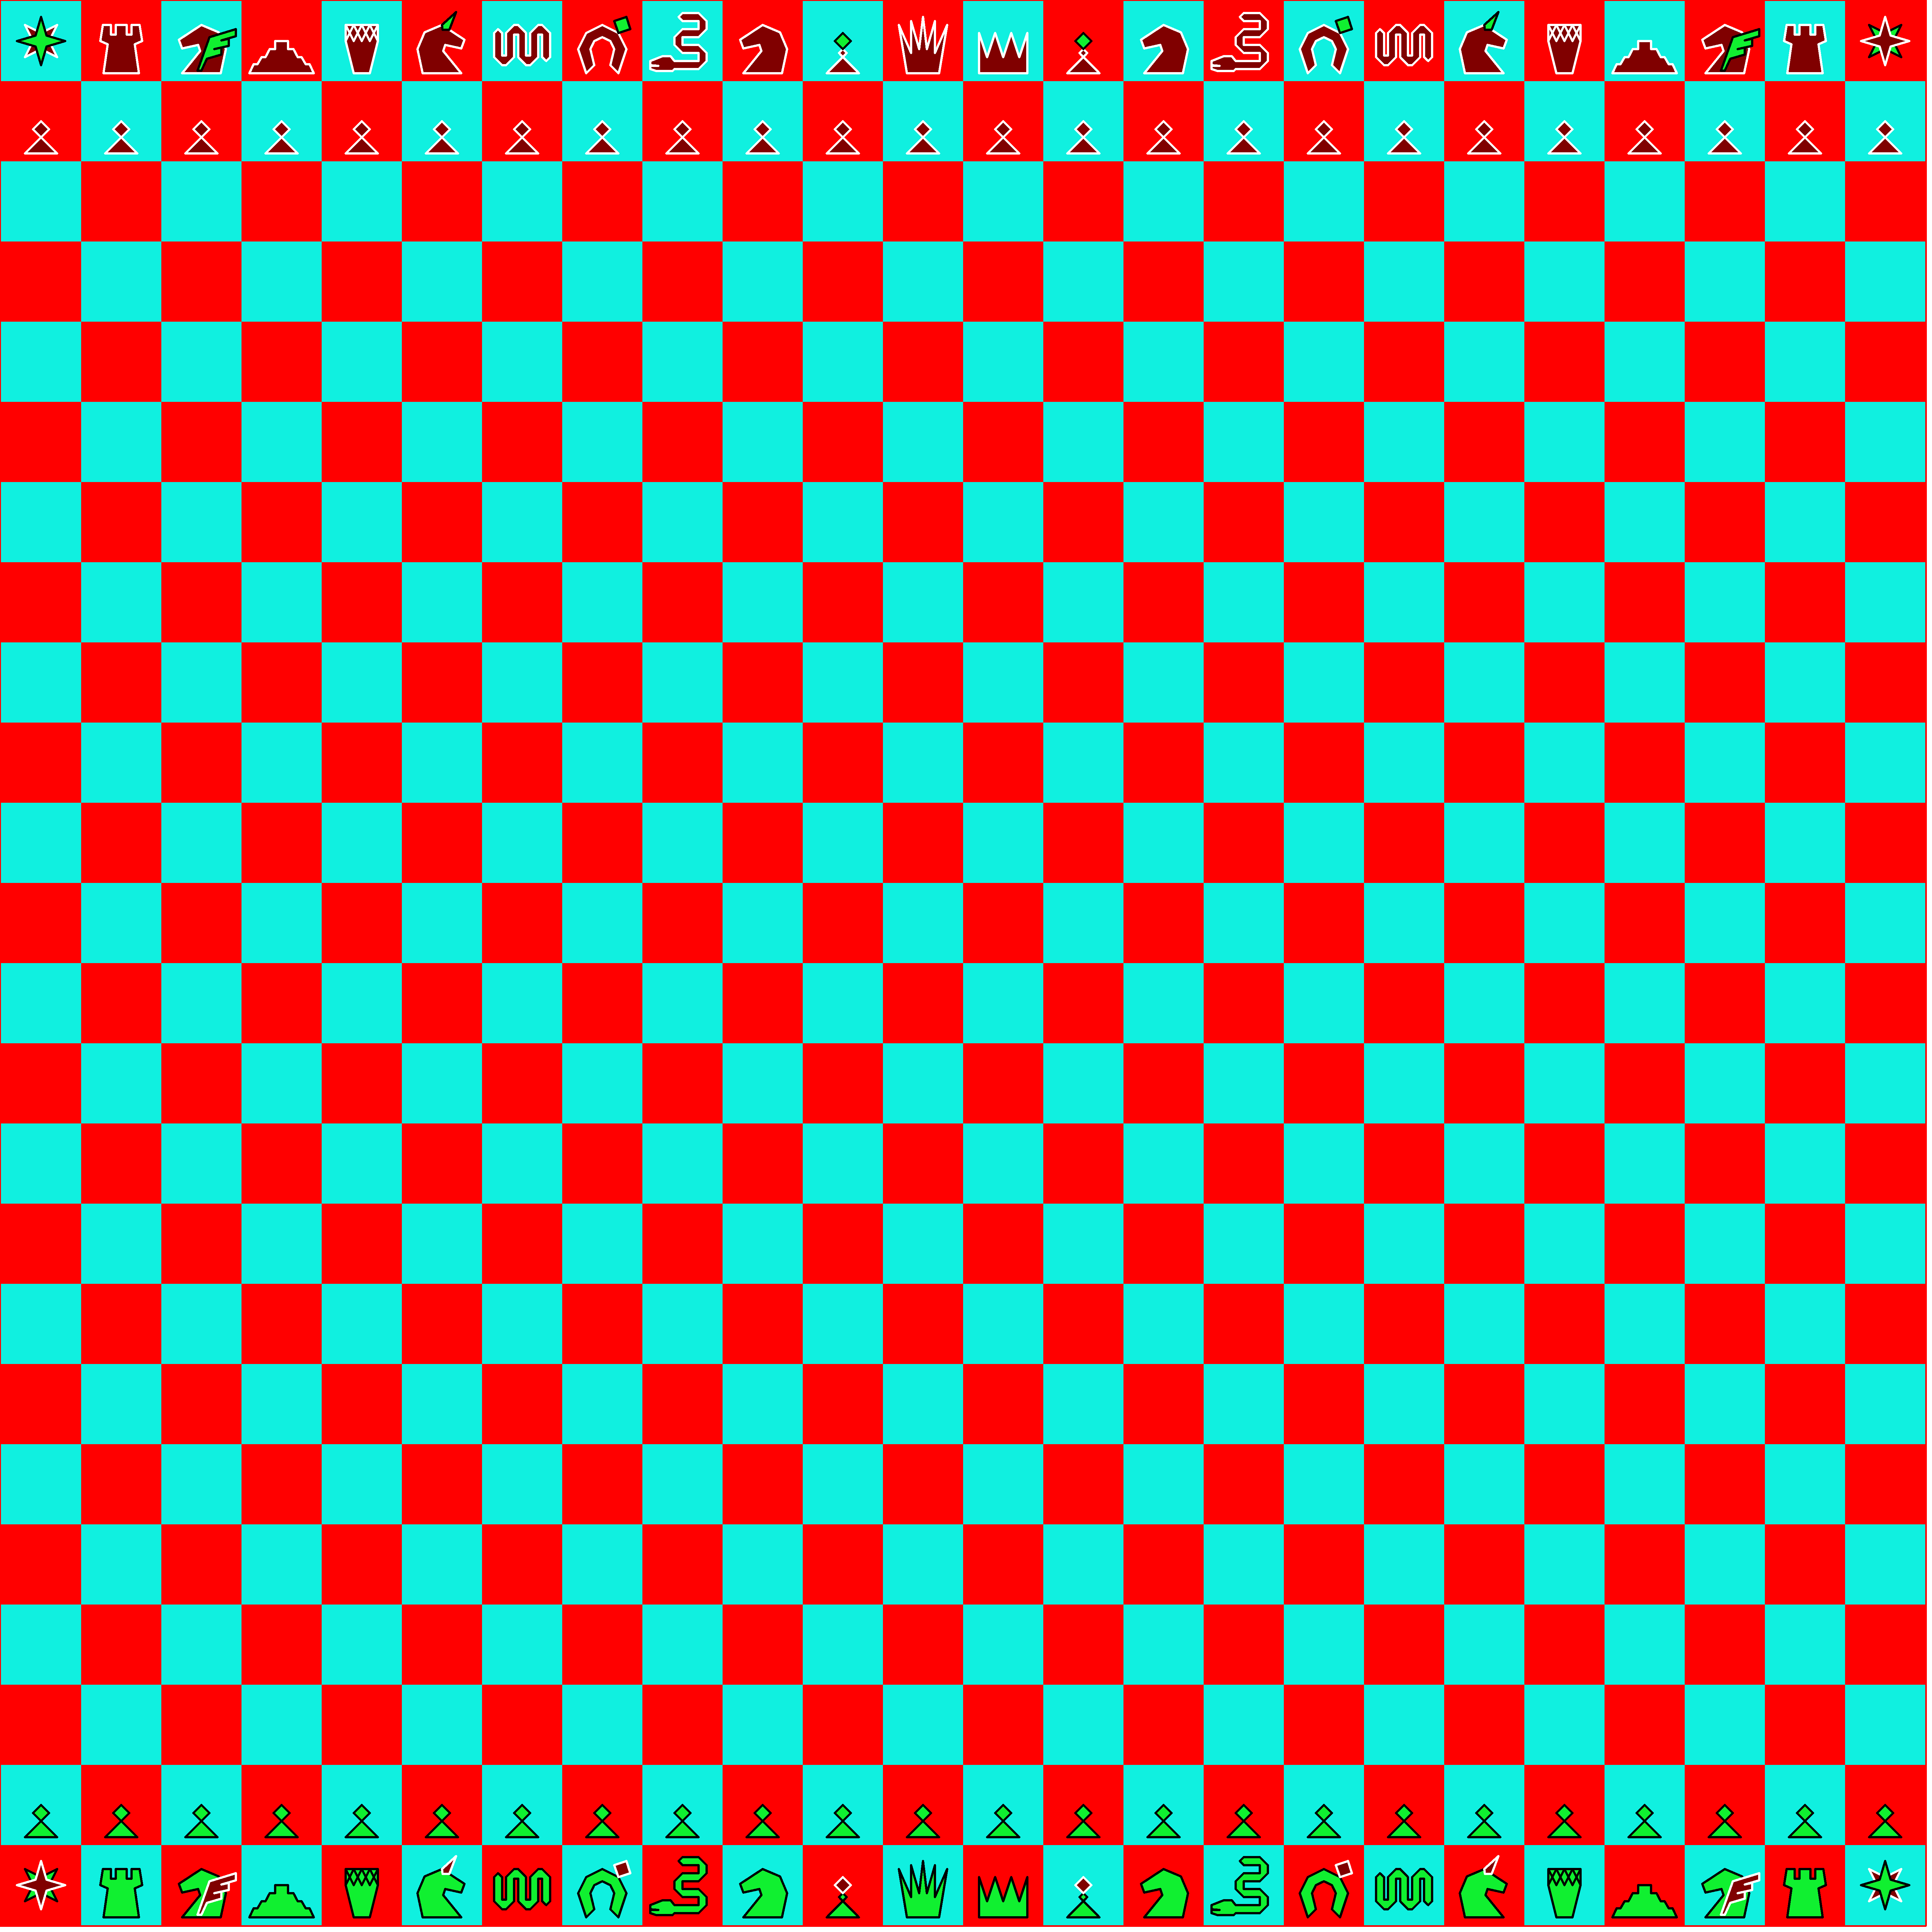
\includegraphics[width=1.0\textwidth, keepaspectratio=true]{boards/18_conquest_of_tlalocan.png}
\caption{Conquest of Tlalocan board}
\label{fig:18_conquest_of_tlalocan}
% \centering
\end{figure}

\clearpage % ..........................................................
% ---------------------------------------- Conquest of Tlalocan chapter
